\documentclass[tikz,border=4pt]{standalone}
\usepackage{amsmath}
\usepackage{tikz}
\usetikzlibrary{arrows.meta,positioning,fit,backgrounds,calc,shapes.geometric,decorations.pathreplacing,patterns}
\usepackage{xcolor}
\renewcommand{\familydefault}{\sfdefault}
\definecolor{cdata}{HTML}{1F5FA8}
\definecolor{cctrl}{HTML}{15796F}
\definecolor{cres}{HTML}{6A4C93}
\definecolor{cgray}{HTML}{5A6570}
\definecolor{cwarn}{HTML}{B4561B}
\tikzset{
  base/.style={rounded corners=1.8pt, line width=0.6pt, align=center, font=\scriptsize, inner sep=3pt, minimum height=8mm, text=black!85},
  data/.style={base, draw=cdata, fill=cdata!9},
  ctrl/.style={base, draw=cctrl, fill=cctrl!9},
  res/.style={base, draw=cres, fill=cres!9},
  art/.style={base, draw=black!65, fill=black!7},
  ext/.style={base, draw=cgray, fill=white, dashed},
  gate/.style={font=\tiny\bfseries, text=cwarn, draw=cwarn, rounded corners=1pt, inner sep=1.6pt, fill=white, line width=0.5pt},
  arr/.style={-{Stealth[length=2.0mm,width=1.5mm]}, line width=0.6pt, draw=cgray!85!black},
  arr2/.style={{Stealth[length=2.0mm,width=1.5mm]}-{Stealth[length=2.0mm,width=1.5mm]}, line width=0.6pt, draw=cgray!85!black},
  darr/.style={-{Stealth[length=2.0mm,width=1.5mm]}, line width=0.6pt, dashed, draw=cgray!85!black},
  lbl/.style={font=\tiny, text=cgray!90!black, inner sep=1pt},
  band/.style={rounded corners=3pt, line width=0.7pt},
}
\newcommand{\dotsep}{\,$\cdot$\,}
\renewcommand{\tiny}{\fontsize{6}{7}\selectfont}

\begin{document}
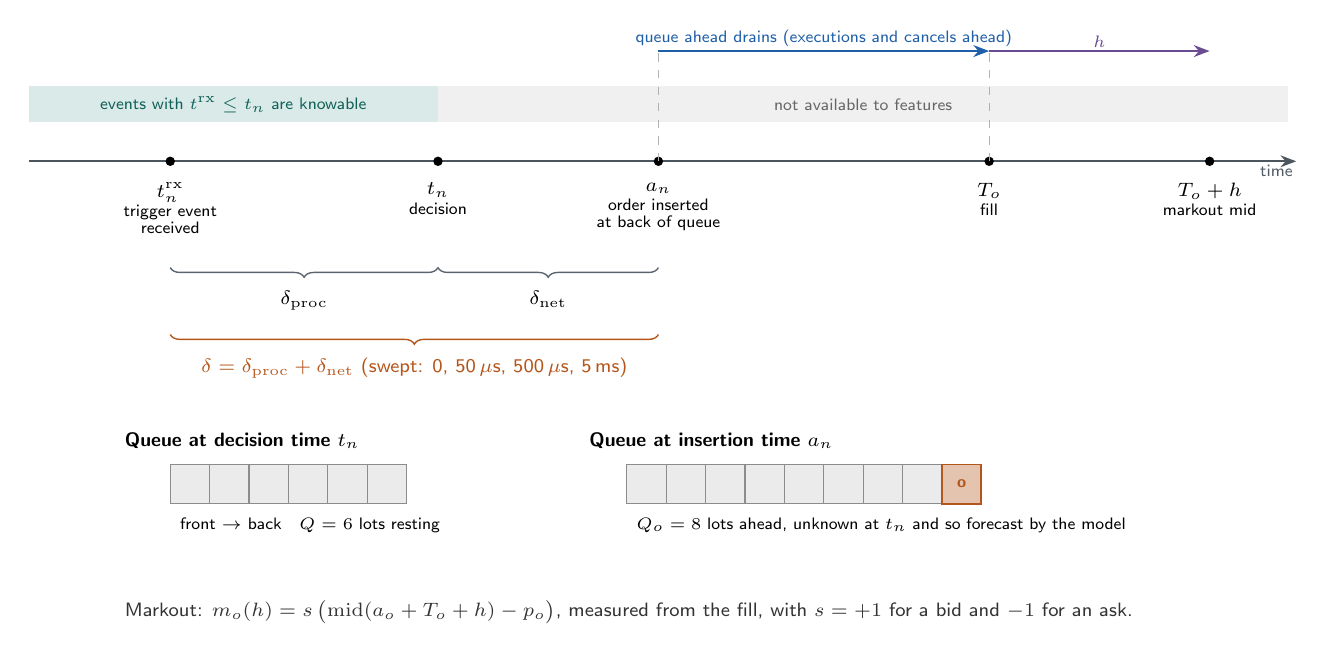
\begin{tikzpicture}
\def\ya{0}
% knowable band
\fill[cctrl!16] (0.4,0.5) rectangle (5.6,0.95);
\fill[black!6]  (5.6,0.5) rectangle (16.4,0.95);
\node[font=\tiny, text=cctrl!80!black] at (3.0,0.72) {events with $t^{\mathrm{rx}} \le t_n$ are knowable};
\node[font=\tiny, text=black!60] at (11.0,0.72) {not available to features};
% axis
\draw[arr] (0.4,0) -- (16.5,0) node[below left, lbl] {time};
\foreach \x in {2.2,5.6,8.4,12.6,15.4}{\fill (\x,0) circle (1.7pt);}
\node[font=\scriptsize, align=center, anchor=north] at (2.2,-0.15) {$t^{\mathrm{rx}}_n$\\[-1pt]\tiny trigger event\\[-2pt]\tiny received};
\node[font=\scriptsize, align=center, anchor=north] at (5.6,-0.15) {$t_n$\\[-1pt]\tiny decision};
\node[font=\scriptsize, align=center, anchor=north] at (8.4,-0.15) {$a_n$\\[-1pt]\tiny order inserted\\[-2pt]\tiny at back of queue};
\node[font=\scriptsize, align=center, anchor=north] at (12.6,-0.15) {$T_o$\\[-1pt]\tiny fill};
\node[font=\scriptsize, align=center, anchor=north] at (15.4,-0.15) {$T_o + h$\\[-1pt]\tiny markout mid};
% fill interval and markout
\draw[arr, line width=0.9pt, draw=cdata] (8.4,1.4) -- node[above, lbl, text=cdata] {queue ahead drains (executions and cancels ahead)} (12.6,1.4);
\draw[arr, line width=0.9pt, draw=cres] (12.6,1.4) -- node[above, lbl, text=cres] {$h$} (15.4,1.4);
\draw[dashed, draw=black!30] (8.4,0) -- (8.4,1.4);
\draw[dashed, draw=black!30] (12.6,0) -- (12.6,1.4);
% delta braces
\draw[decorate, decoration={brace, mirror, amplitude=3.5pt}, line width=0.5pt, draw=cgray] (2.2,-1.35) -- (5.6,-1.35) node[midway, below=5pt, font=\scriptsize] {$\delta_{\mathrm{proc}}$};
\draw[decorate, decoration={brace, mirror, amplitude=3.5pt}, line width=0.5pt, draw=cgray] (5.6,-1.35) -- (8.4,-1.35) node[midway, below=5pt, font=\scriptsize] {$\delta_{\mathrm{net}}$};
\draw[decorate, decoration={brace, mirror, amplitude=3.5pt}, line width=0.5pt, draw=cwarn] (2.2,-2.2) -- (8.4,-2.2) node[midway, below=5pt, font=\scriptsize, text=cwarn] {$\delta = \delta_{\mathrm{proc}} + \delta_{\mathrm{net}}$ (swept: 0, 50\,$\mu$s, 500\,$\mu$s, 5\,ms)};
% queues
\def\c{0.5}
\node[font=\scriptsize\bfseries, anchor=west] at (1.5,-3.55) {Queue at decision time $t_n$};
\foreach \i in {0,...,5}{\draw[fill=black!8, draw=black!45, line width=0.4pt] (2.2+\i*\c,-4.35) rectangle (2.2+\i*\c+\c,-3.85);}
\node[font=\tiny, anchor=north west] at (2.2,-4.4) {front $\rightarrow$ back\quad $Q = 6$ lots resting};
\node[font=\scriptsize\bfseries, anchor=west] at (7.4,-3.55) {Queue at insertion time $a_n$};
\foreach \i in {0,...,7}{\draw[fill=black!8, draw=black!45, line width=0.4pt] (8.0+\i*\c,-4.35) rectangle (8.0+\i*\c+\c,-3.85);}
\draw[fill=cwarn!35, draw=cwarn, line width=0.6pt] (8.0+8*\c,-4.35) rectangle (8.0+9*\c,-3.85);
\node[font=\tiny\bfseries, text=cwarn] at (8.0+8.5*\c,-4.1) {o};
\node[font=\tiny, anchor=north west, align=left] at (8.0,-4.4) {$Q_o = 8$ lots ahead, unknown at $t_n$ and so forecast by the model};
\node[font=\scriptsize, anchor=north west, text=black!80] at (1.5,-5.45) {Markout: $m_o(h) = s\,\bigl(\mathrm{mid}(a_o + T_o + h) - p_o\bigr)$, measured from the fill, with $s=+1$ for a bid and $-1$ for an ask.};
\end{tikzpicture}
\end{document}
